%To compile as handout, use
%pdflatex "\def\ishandout{1} \input{filename.tex}"
%Defaults to non-handout mode (with slide reveals)
\ifdefined\ishandout
  \documentclass[handout]{beamer}
\else
  \documentclass{beamer}
\fi
 
\usepackage{econ103slides} 

\date{Lecture 22}


\begin{document} 





%%%%%%%%%%%%%%%%%%%%%%%%%%%%%%%%%%%%%%%%

\begin{frame}[plain]
	\titlepage 
	

\end{frame} 



%%%%%%%%%%%%%%%%%%%%%%%%%%%%%%%%%%%%%%%%

\begin{frame}
\frametitle{Hypothesis Testing Part III}
	\begin{enumerate}
\item Example: Which Exam was Harder?
\item Relationship Between Testing and CIs
\item Tests for Proportions 
\item \alert{Statistical Power}
\end{enumerate}
\end{frame}

%%%%%%%%%%%%%%%%%%%%%%%%%%%%%%%%%%%%%%%%
\begin{frame}
\frametitle{Which Exam is Harder?}
% latex.default(round(grades.out, 1), file = "grades.tex", rowname = NULL) 
%
\begin{table}[!tbp]
\begin{center}
\begin{tabular}{rccr}
\hline\hline
\multicolumn{1}{r}{Student}&\multicolumn{1}{c}{Exam 1}&\multicolumn{1}{c}{Exam 2}&\multicolumn{1}{r}{Difference}\tabularnewline
\hline
$ 1$&$57.1$&$60.7$&$  3.6$\tabularnewline
\vdots&\vdots&\vdots&\vdots\\
$71$&$78.6$&$82.9$&$  4.3$\tabularnewline
\hline
Sample Mean: & 79.6 & 81.4  &1.8\\
Sample Var. &117  & 151 & 124\\
Sample Corr.& \multicolumn{2}{c}{0.54}&\\
\hline
\end{tabular}
\end{center}
\end{table}

\end{frame}
%%%%%%%%%%%%%%%%%%%%%%%%%%%%%%%%%%%%%%%%
\begin{frame}
\frametitle{One-Sample Hypothesis Test Using Differences}
\small
\fbox{Let $D_i = X_i - Y_i$ be (Midterm 2 Score - Midterm 1 Score) for student $i$}
\vspace{0.1em}
\begin{block}{Null Hypothesis}
$H_0\colon \mu_1 = \mu_2$, i.e.\ both exams were of the same difficulty
\end{block}
\begin{block}{Two-Sided Alternative}
$H_1\colon \mu_1 \neq \mu_2$, i.e.\ one exam was harder than the other
\end{block}
\begin{block}{One-Sided Alternative}
$H_1\colon \mu_2 > \mu_1$, i.e.\ the second exam was easier
\end{block}
% \begin{block}{Test Statistic}
% Under $H_0$ this has an approx.\ standard normal distribution by the CLT:
% 	$$\displaystyle \frac{\bar{D}_n}{\widehat{SE}(\bar{D}_n)}=  \frac{1.8}{\sqrt{124/71}}  \approx \alert{1.36} $$
% \end{block}
%\alert{Approximate 95\% CI Based on the CLT:}
%$$\alert{\boxed{1.8 \pm 2.6 = (-0.8, 4.4)}} \quad \mbox{What is our conclusion?}$$

\end{frame}
%%%%%%%%%%%%%%%%%%%%%%%%%%%%%%%%%%%%%%%%

\begin{frame}
\frametitle{Decision Rules}
\small
\fbox{Let $D_i = X_i - Y_i$ be (Midterm 2 Score - Midterm 1 Score) for student $i$}
\vspace{0.1em}


\begin{block}
	{Test Statistic}
$$\displaystyle \frac{\bar{D}_n}{\widehat{SE}(\bar{D}_n)}=\frac{1.8}{\sqrt{124/71}} \approx 1.36$$
\end{block}


\begin{block}{Two-Sided Alternative} 
Reject $H_0\colon \mu_1 = \mu_2$ in favor of $H_1\colon \mu_1 \neq \mu_2$ if $|\bar{D}_n|$ is sufficiently large.
\end{block}
\begin{block}{One-Sided Alternative}
Reject $H_0\colon \mu_1 = \mu_2$ in favor of $H_1\colon \mu_2 >\mu_1$ if $\bar{D}_n$ is sufficiently large.
\end{block}
\end{frame}
%%%%%%%%%%%%%%%%%%%%%%%%%%%%%%%%%%%%%%%%

\begin{frame}
\frametitle{Reject against \emph{Two-sided} Alternative with $\alpha = 0.1$?  
\includegraphics[scale = 0.05]{./images/clicker}}

	$$\boxed{\displaystyle \frac{\bar{D}_n}{\widehat{SE}(\bar{D}_n)}= \frac{1.8}{\sqrt{124/71}} \approx 1.36} $$

\begin{center}
\begin{tabular}{l|lll}
$\alpha$ &   0.10& 0.05 &0.01\\
\hline
\texttt{qnorm($1-\alpha$)} & 1.28 &1.64 &2.33\\
\texttt{qnorm($1-\alpha/2$)} &1.64 &1.96& 2.58
\end{tabular}
\end{center}

\begin{enumerate}[(a)]
\item Reject
\item Fail to Reject
\item Not Sure
\end{enumerate}

\end{frame}

%%%%%%%%%%%%%%%%%%%%%%%%%%%%%%%%%%%%%%%%
\begin{frame}
\frametitle{Reject against \emph{One-sided} Alternative with $\alpha = 0.1$?  
\includegraphics[scale = 0.05]{./images/clicker}}

	$$\boxed{\displaystyle \frac{\bar{D}_n}{\widehat{SE}(\bar{D}_n)}= \frac{1.8}{\sqrt{124/71}} \approx 1.36} $$

\begin{center}
\begin{tabular}{l|lll}
$\alpha$ &   0.10& 0.05 &0.01\\
\hline
\texttt{qnorm($1-\alpha$)} & 1.28 &1.64 &2.33\\
\texttt{qnorm($1-\alpha/2$)} &1.64 &1.96& 2.58
\end{tabular}
\end{center}

\begin{enumerate}[(a)]
\item Reject
\item Fail to Reject
\item Not Sure
\end{enumerate}



\end{frame}

%%%%%%%%%%%%%%%%%%%%%%%%%%%%%%%%%%%%%%%%
\begin{frame}
\frametitle{P-Values for the Test of $H_0\colon \mu_1 = \mu_2$}

	$$\boxed{\displaystyle \frac{\bar{D}_n}{\widehat{SE}(\bar{D}_n)}= \frac{1.8}{\sqrt{124/71}} \approx 1.36} $$

\begin{block}{One-Sided $H_1\colon \mu_2 > \mu_1 $} 
$\texttt{1 - pnorm(1.36)} =  \texttt{pnorm(-1.36)}  \approx 0.09$ 
\end{block}

\begin{block}{Two-Sided $H_1 \colon \mu_1 \neq \mu_2$} 
$\texttt{2 * (1 - pnorm(1.36))} =  \texttt{2 * pnorm(-1.36)} \approx 0.18$
\end{block}
\end{frame}
%%%%%%%%%%%%%%%%%%%%%%%%%%%%%%%%%%%%%%%%


\begin{frame}
\frametitle{Relationship between CI and Two-sided Test}
Suppose $X_1, \hdots, X_n \sim \mbox{iid } N(\mu,\sigma^2)$

\vspace{1em}
	\begin{block}{Test $H_0\colon \mu = \mu_0$ vs.\ $H_1\colon \mu \neq \mu_0$ at significance level $\alpha$} 
		\begin{itemize}
			\item Test Statistic:  $T_n = \sqrt{n}(\bar{X}_n - \mu_0)/S \sim t(n-1)$ under $H_0$ 
			\item Decision Rule: Reject $H_0$ if $|T_n| > \texttt{qt}(1-\alpha/2, \texttt{df}=n-1)$ 
			\end{itemize}

			\pause
\end{block}
	\begin{block}{$100\times (1-\alpha)\%$ CI for $\mu$} 
		$$\bar{X}_n \pm \texttt{qt}(1-\alpha/2, \texttt{df}=n-1) \frac{S}{\sqrt{n}}$$
\end{block}
\end{frame}
%%%%%%%%%%%%%%%%%%%%%%%%%%%%%%%%%%%%%%%%
\begin{frame}
\frametitle{Relationship between CI and Two-sided Test}
$\alert{c =  \texttt{qt}(1-\alpha/2, \texttt{df}=n-1)}$
\begin{block}{Decision Rule: Reject $H_0$ if}
		$$\left|\frac{\bar{X}_n - \mu_0}{S/\sqrt{n}} \right|> c \quad \iff \pause  \quad \left(\frac{\bar{X}_n - \mu_0}{S/\sqrt{n}}> c \;\;\mbox{  \alert{OR}  }\;\;\frac{\bar{X}_n - \mu_0}{S/\sqrt{n}}< - c\right)$$
\end{block}

\pause
\begin{block}{Equivalent to: \emph{Don't Reject} $H_0$ provided}
	$$-c \leq \frac{\bar{X}_n - \mu_0}{S/\sqrt{n}}\leq c $$ \pause
	$$\alert{\bar{X_n} - c\times \frac{S}{\sqrt{n}} \leq \mu_0 \leq \bar{X_n} + c\times \frac{S}{\sqrt{n}}}$$
\end{block}
\end{frame}
%%%%%%%%%%%%%%%%%%%%%%%%%%%%%%%%%%%%%%%%
\begin{frame}
\frametitle{What does this mean?}

\begin{block}
	{Two-sided Test $\iff$ Checking if $\mu_0 \in$ CI}
	A two-sided test of $H_0\colon \mu = \mu_0$ against $H_1\colon \mu\neq \mu_0 $ at significance level $\alpha$ is equivalent to checking whether $\mu_0$ lies inside the corresponding $100\times (1-\alpha)\%$ confidence interval for $\mu$.
\end{block}

\pause

\begin{block}
	{``Inverting'' Two-sided Test to get a CI}	
	Collect all the values $\mu_0$ such that we cannot reject $H_0\colon \mu = \mu_0$ against the two-sided alternative. The result is \emph{precisely} a $100\times (1-\alpha)\%$ CI for $\mu$.
\end{block}
\end{frame}
%%%%%%%%%%%%%%%%%%%%%%%%%%%%%%%%%%%%%%%%

\begin{frame}
\frametitle{Tests and CIs for Proportions}
\footnotesize
Suppose $X_1, \hdots, X_n \sim \mbox{iid Bernoulli}(p)$ indep.\ of $Y_1, \hdots, Y_m \sim \mbox{iid Bernoulli}(q)$.\\
\normalsize
\vspace{1em}

From the CLT:
	$$\frac{\hat{p} - p}{\sqrt{\frac{\hat{p}(1-\hat{p})}{n}}} \approx N(0,1)$$
and
$$\frac{(\hat{p} - \hat{q}) - (p-q)}{\sqrt{\frac{\hat{p}(1-\hat{p})}{n} + \frac{\hat{q}(1-\hat{q})}{m}}} \approx N(0,1)$$

\alert{We can use these results for both testing and building CIs}
\end{frame}
%%%%%%%%%%%%%%%%%%%%%%%%%%%%%%%%%%%%%%%%
\begin{frame}
\frametitle{``Textbook'' CIs for Proportions}
	$$\widehat{p} \pm \texttt{qnorm}(1 - \alpha/2) \times \sqrt{\frac{\hat{p}(1-\hat{p})}{n}}$$
	
	$$\left(\widehat{p} -\widehat{q}\right)\pm \texttt{qnorm}(1 - \alpha/2) \times \sqrt{\frac{\hat{p}(1-\hat{p})}{n} + \frac{\hat{q}(1-\hat{q})}{m}}$$
\end{frame}
%%%%%%%%%%%%%%%%%%%%%%%%%%%%%%%%%%%%%%%%
\begin{frame}
	\frametitle{``Unrefined'' Tests for Proportions -- Like Tests for Means}
	$$H_0\colon p = p_0 \Rightarrow \frac{\hat{p} - p_0}{\sqrt{\frac{\hat{p}(1-\hat{p})}{n}}} \approx N(0,1)$$
	\vspace{1em}
	
	$$H_0\colon p = q \Rightarrow \frac{\hat{p} - \hat{q}}{\sqrt{\frac{\hat{p}(1-\hat{p})}{n} + \frac{\hat{q}(1-\hat{q})}{m}}} \approx N(0,1)$$
\end{frame}
%%%%%%%%%%%%%%%%%%%%%%%%%%%%%%%%%%%%%%%%
\begin{frame}
\frametitle{Refined Tests for Proportions: Fully Impose $H_0$}

\begin{block}{Under $H_0$ we know something about the standard error!}
For proportions, mean and SE are are linked!
\end{block}
\begin{block}{One-sample: SE Known under $H_0$}
	$$H_0\colon p = p_0 \Rightarrow \frac{\hat{p} - p_0}{\sqrt{\frac{p_0(1-p_0)}{n}}} \approx N(0,1)$$
\end{block}
	\pause
\begin{block}{Two-sample: Pooled SE estimator under $H_0$}
	$$H_0\colon p = q \Rightarrow \frac{\hat{p} - \hat{q}}{\sqrt{\left(\frac{1}{n} + \frac{1}{m} \right)\widehat{\pi}(1-\widehat{\pi})}} \approx N(0,1)$$
	where $\widehat{\pi} = \frac{n\widehat{p} + m\widehat{q}}{n+m}$
\end{block}
\end{frame}
%%%%%%%%%%%%%%%%%%%%%%%%%%%%%%%%%%%%%%%%
% \begin{frame}
% \frametitle{Refined Test and Refined CI}
% \small
% \begin{block}{Refined Test Imposes $H_0$ in \emph{both} Numerator \& Denominator}
% Our procedures for proportions are approximations based on the CLT. (The population in question is actually Bernoulli!) Fully imposing the null, as on the previous slide, makes the approximation work better.
% \end{block}

% \pause

% \begin{block}{Ideally Invert Refined Test to get CI}
% Earlier in this lecture, we talked about how the set of all parameter values that are not rejected by a two-sided test with significance level $\alpha$ gives a $100\times(1-\alpha)\%$ CI. Ideally, we could invert the refined tests for proportions to get \emph{corresponding} refined CIs. The math required for this, however, is a little tricky.
% \end{block}

% \end{frame}
% %%%%%%%%%%%%%%%%%%%%%%%%%%%%%%%%%%%%%%%%
\begin{frame}
	\frametitle{``Refined'' Procedures for Proportions}
\begin{columns}
	\column{0.45\textwidth}
	\begin{block}
		{Refined CI}
		Add four ``fake'' observations.
	\end{block}
	\column{0.45\textwidth}
		\begin{block}
			{Refined Test} Fully impose $H_0$ in $T_n$
		\end{block}
\end{columns}

\vspace{2em}

\begin{block}
	{What's Going on Here?}
		\begin{itemize}
		\item $X_1, \hdots, X_n \sim \mbox{ iid Bernoulli}(p)$ has special structure:
			\begin{enumerate}
				\item Discrete Data (zeros and ones)
				\item Single Population parameter $p$ 
			\end{enumerate}
		\item Use this structure to improve the approximation of the CLT
		\item Turns out that the refined CI is approximately what you get from inverting the corresponding refined test.
	\end{itemize}
\end{block}
\end{frame}

%%%%%%%%%%%%%%%%%%%%%%%%%%%%%%%%%%%%%%%%
% \begin{frame}
% \frametitle{Refined Test and Refined CI}
% \small
% \begin{block}{Inverting \emph{Unrefined Tests} Gives Textbook CI}
% The \emph{unrefined} tests for proportions do not use the fact that, under the null, we actually have some additional information regarding the standard errors. If we invert these tests, we get the textbook confidence intervals studied earlier (see preceding slides). 
% \end{block}

% \pause

% \begin{block}{Refined CIs are an \emph{Approximation} to Inverting Refined Tests}
% A few lectures ago, we talked about the refined CIs for proportions that involved adding ``fake'' observations to the data. These are \emph{very close} to what you get if you inverted the refined tests. \alert{This is why we use them.}
% \end{block}

% \pause

% \vspace{1em} 
% \large
% \alert{Unless instructed otherwise, you should \emph{always} use the refined tests and refined CIs when working with proportions: they work better.}

% \end{frame}
% %%%%%%%%%%%%%%%%%%%%%%%%%%%%%%%%%%%%%%%%
\begin{frame}
\frametitle{What is a Type I Error? 
\includegraphics[scale = 0.05]{./images/clicker}}

\begin{enumerate}[(a)]
	\item Rejecting a false Null
	\item Failing to Reject a True Null
	\item Rejecting a True Null
	\item Failing to Reject a False Null
\end{enumerate}

\end{frame}


%%%%%%%%%%%%%%%%%%%%%%%%%%%%%%%%%%%%%%%%
\begin{frame}
\frametitle{What is a Type II Error? 
\includegraphics[scale = 0.05]{./images/clicker}}

\begin{enumerate}[(a)]
	\item Rejecting a False Null
	\item Failing to Reject a True Null
	\item Rejecting a True Null
	\item Failing to Reject a False Null
\end{enumerate}

\end{frame}


%%%%%%%%%%%%%%%%%%%%%%%%%%%%%%%%%%%%%%%%
% \begin{frame}
% \frametitle{Which is the Probability of a Type I Error? 
\includegraphics[scale = 0.05]{./images/clicker}}

% \begin{enumerate}[(a)]
% 	\item $\beta$
% 	\item $1 - \beta$
% 	\item $1-\alpha$
% 	\item $\alpha$
% \end{enumerate}

% \end{frame}
%%%%%%%%%%%%%%%%%%%%%%%%%%%%%%%%%%%%%%%%
\begin{frame}[c]\frametitle{The Power of a Test}
    
\begin{block}
	{Type I Error} Rejecting $H_0$ when it is true:  $P(\mbox{Type I Error}) = \alpha$
\end{block}

\begin{block}
	{Type II Error} Failing to reject $H_0$ when it is false: \alert{$P(\mbox{Type II Error}) =\beta$}
\end{block}

\begin{alertblock}
	{Statistical Power} The probability of rejecting $H_0$ when it is false: \alert{$\mbox{Power} = 1 -\beta $}\\ i.e.\ the probability of \emph{convicting} a guilty person.
\end{alertblock}

\vspace{1em}

\begin{center}
\alert{\boxed{
\begin{minipage}
	{0.95\textwidth}
	Hypothesis tests designed to control Type I error rate ($\alpha$). But we also care about Type II errors. What can learn about these?
\end{minipage}}}
\end{center}
\end{frame}
%%%%%%%%%%%%%%%%%%%%%%%%%%%%%%%%%%%%%%%%
\begin{frame}
\frametitle{Example of Calculating Power: Is this coin fair?}

\begin{block}
{Flip a Possibly Unfair Coin $n$ Times}
$X_1, \hdots, X_n \sim \mbox{iid Bernoulli}(p)$ where $p$ may not equal 1/2
\end{block}

\begin{block}
	{Test $H_0\colon p = 0.5$ against $H_1\colon p \neq 0.5$}
	Under $H_0$ and if $n$ is large the CLT gives 
	$$\displaystyle T_n = \frac{\widehat{p} - 0.5}{\sqrt{\frac{0.5(1-0.5)}{n}}}\approx N(0,1)$$
\end{block}

\begin{alertblock}
	{The Idea Behind Statistical Power}
	How does the test statistic behave if the  $H_0$ is \emph{false}? What is the sampling distribution of $T_n$ \emph{under the alternative}: $H_1\colon p\neq 0.5$
\end{alertblock}

\end{frame}
%%%%%%%%%%%%%%%%%%%%%%%%%%%%%%%%%%%%%%%%
\begin{frame}
% \frametitle{Sampling Dist.\ of $T_n$ Under the Alternative $H_1\colon p \neq 0.5$}

\begin{block}
	{Key Distributional Result}
	Center and standardize $\widehat{p}$ using \emph{true} $p \implies$ standard normal:
	$$Z = \frac{\widehat{p} - p}{\sqrt{\frac{p(1-p)}{n}}}  \approx N(0,1)$$
\end{block}

\begin{block}
	{Under the Alternative $p\neq 0.5$}
	$T_n$ is \emph{incorrectly centered and scaled}: $\displaystyle T_n = \frac{\widehat{p} - 0.5}{\sqrt{\frac{0.5(1-0.5)}{n}}} \neq N(0,1)$
\end{block}

\begin{alertblock}
	{How We'll Proceed}
	Use algebra to express $T_n$ in terms of $Z$, which we know is $N(0,1)$, and constants. This will give the distribution of $T_n$ under $H_1$.
\end{alertblock}
\end{frame}
%%%%%%%%%%%%%%%%%%%%%%%%%%%%%%%%%%%%%%%%
\begin{frame}
\frametitle{This is Just Algebra}
\small
	\begin{eqnarray*}
	T_n &=&\frac{\widehat{p} - 0.5}{\sqrt{\frac{0.5(1-0.5)}{n}}} =\sqrt{n}(2\widehat{p} - 1)\\ \\
	&=& \sqrt{n} \left[2\widehat{p} -1 + (2p -2p)\right] = \sqrt{n}\left[ 2\left(\widehat{p} - p\right) + 2p -1\right]\\ \\
	&=& \sqrt{n}\left[ 2\left(\widehat{p} - p\right) \left(\frac{\sqrt{p(1-p)/n}}{\sqrt{p(1-p)/n}}\right) + 2p -1\right]\\ \\
		&=& \sqrt{n}\left[ 2\sqrt{\frac{p(1-p)}{n}} \alert{\left(\frac{\widehat{p} - p}{\sqrt{p(1-p)/n}}\right)} + 2p -1\right]\\ \\
		&=& \left[2\sqrt{p(1-p)}\right] \alert{Z} + \sqrt{n}(2p -1)\\
		&=& a\, \alert{Z} + b
\end{eqnarray*}
\end{frame}
%%%%%%%%%%%%%%%%%%%%%%%%%%%%%%%%%%%%%%%%
\begin{frame}
\frametitle{Distribution of Test Statistic Under $H_1\colon p \neq 0.5$ }

From the previous slide,
	$$T_n =\frac{\widehat{p} - 0.5}{\sqrt{\frac{0.5(1-0.5)}{n}}} = \alert{a Z + b}$$
where:
	\begin{eqnarray*}
		Z &=& \frac{\widehat{p} - p}{\sqrt{p(1-p)/n}} \approx N(0,1)\\ 
		a &=& 2\sqrt{p(1-p)}\\ 
		b &=& \sqrt{n}(2p -1) 
	\end{eqnarray*}

\vspace{1em}
\alert{Hence: $T_n \approx N(\mu = b, \sigma^2 = a^2)$}
\end{frame}
%%%%%%%%%%%%%%%%%%%%%%%%%%%%%%%%%%%%%%%%
\begin{frame}[c]\frametitle{Distribution of $T_n$ Under the Alternative}
    
    $$\boxed{T_n =\frac{\widehat{p} - 0.5}{\sqrt{\frac{0.5(1-0.5)}{n}}} \approx N\left(\sqrt{n}(2p-1), 4p(1-p) \right)}$$

\begin{block}
	{Note That:}
	\begin{enumerate}
		\item Mean depends on $p$ and $n$
		\item Variance depends only on $p$
		\item If $p=0.5$ so $H_0$ is true, this reduces to a standard normal:
		\begin{eqnarray*}
		\mbox{Mean} &=&  \sqrt{n}(2p-1) = \sqrt{n}(2\times 1/2 - 1) = 0\\
			\mbox{Variance} &=& 4p(1-p) = 4 \times 1/2 \times (1 - 1/2) = 1\\
		\end{eqnarray*}
	\end{enumerate}
\end{block}

\end{frame}

%%%%%%%%%%%%%%%%%%%%%%%%%%%%%%%%%%%%%%%%
\begin{frame}
	\frametitle{\href{http://glimmer.rstudio.com/fditraglia/power_proptest/}{http://glimmer.rstudio.com/fditraglia/power\_proptest/}}
\framesubtitle{Ignore everything except the solid curve and play around with the first two sliders.}

\begin{figure}
	\fbox{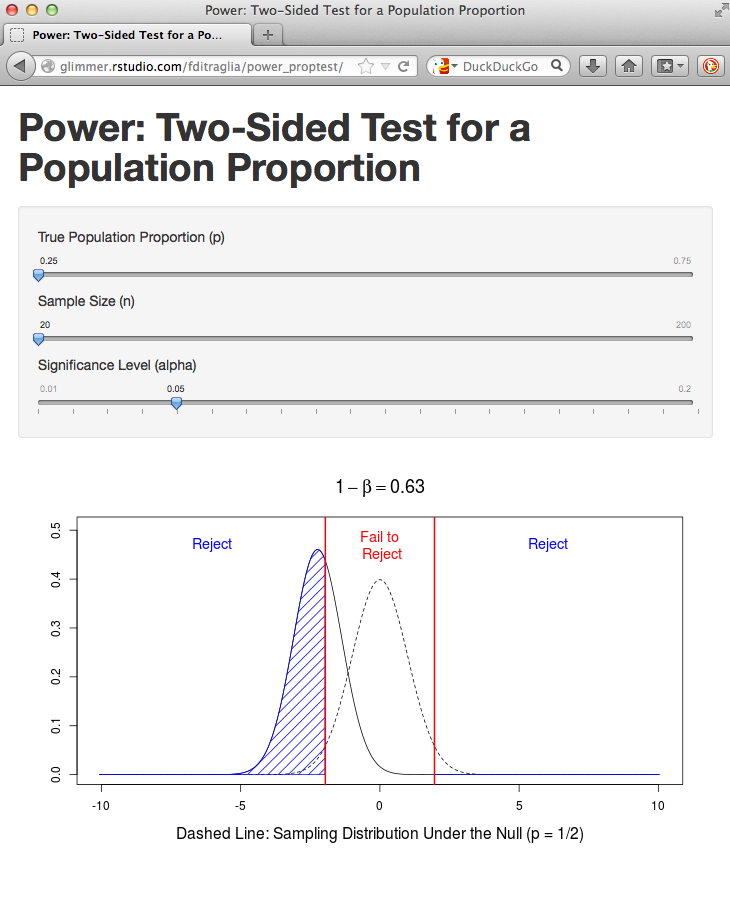
\includegraphics[scale = 0.22]{./images/power_proptest_screenshot}}
\end{figure}

\end{frame}
%%%%%%%%%%%%%%%%%%%%%%%%%%%%%%%%%%%%%%%%
\begin{frame}
\frametitle{Now We can Calculate Power!}
\small
\begin{block}{Decision Rule for Two-sided Test}
Reject $H_0\colon p = 0.5$ provided that $\alert{|T_n| \geq \texttt{qnorm}(1 - \alpha/2)}$
\end{block}

\begin{block}{If the null is false (i.e.\ under $H_1\colon p \neq 0.5$)}
	$$T_n = \frac{\widehat{p} - 0.5}{\sqrt{\frac{0.5(1-0.5)}{n}}} \approx N\left(\sqrt{n}(2p-1), 4 p(1-p)  \right)$$
\end{block}
\begin{block}{Thus, the probability of rejecting a false null is:}
	$$\boxed{\mbox{Power}(\alpha, p, n) = P\left( |Y| \geq c\right)  = P(Y \leq -c) + P(Y\geq c)}$$
		\begin{eqnarray*}
			 c &=&\texttt{qnorm}(1 - \alpha/2) \\
			 Y &\sim& N\left(\sqrt{n}(2p-1), 4 p(1-p)  \right)
		 \end{eqnarray*} 
\end{block}
\end{frame}
%%%%%%%%%%%%%%%%%%%%%%%%%%%%%%%%%%%%%%%%
\begin{frame}
	\frametitle{\href{http://glimmer.rstudio.com/fditraglia/power_proptest/}{http://glimmer.rstudio.com/fditraglia/power\_proptest/}}
\framesubtitle{Now look at everything and try changing all the sliders!}

\begin{figure}
	\fbox{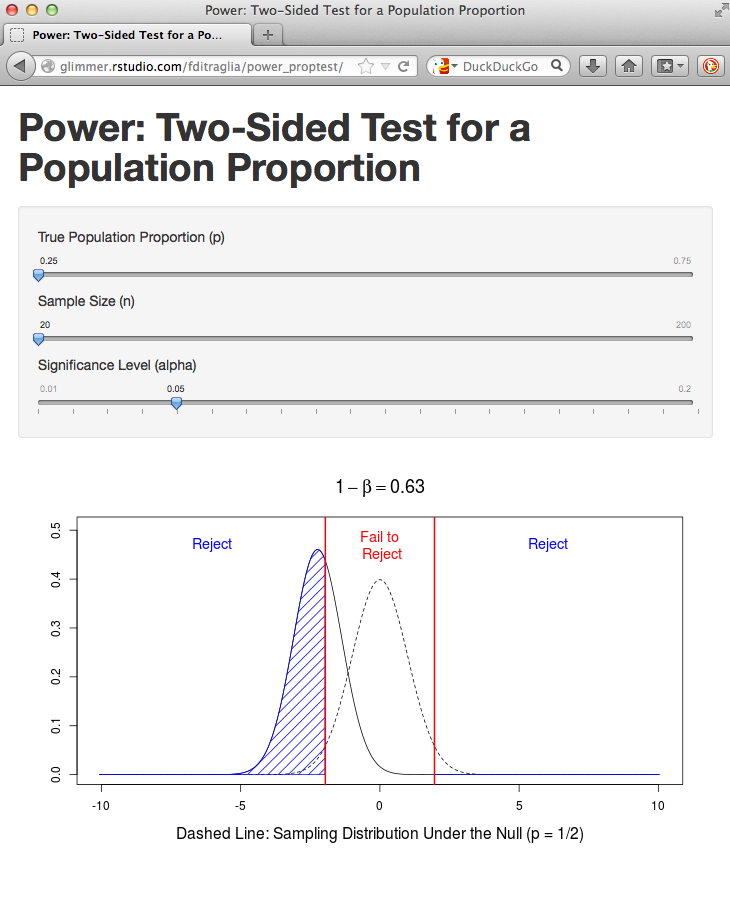
\includegraphics[scale = 0.22]{./images/power_proptest_screenshot}}
\end{figure}

\end{frame}
%%%%%%%%%%%%%%%%%%%%%%%%%%%%%%%%%%%%%%%%\begin{frame}
\begin{frame}
\begin{center}
	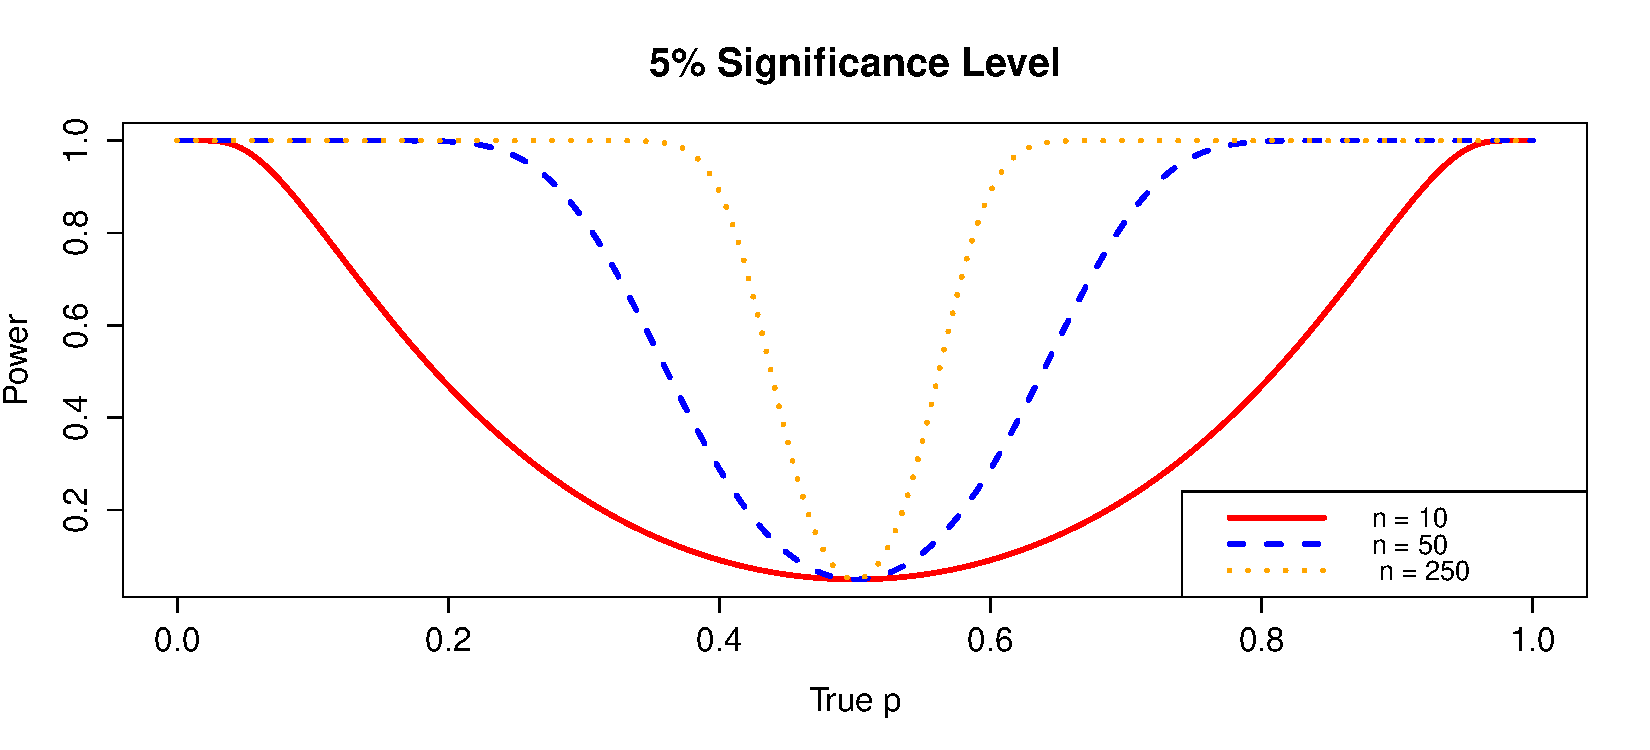
\includegraphics[scale=0.37]{./images/power_change_n}\\
	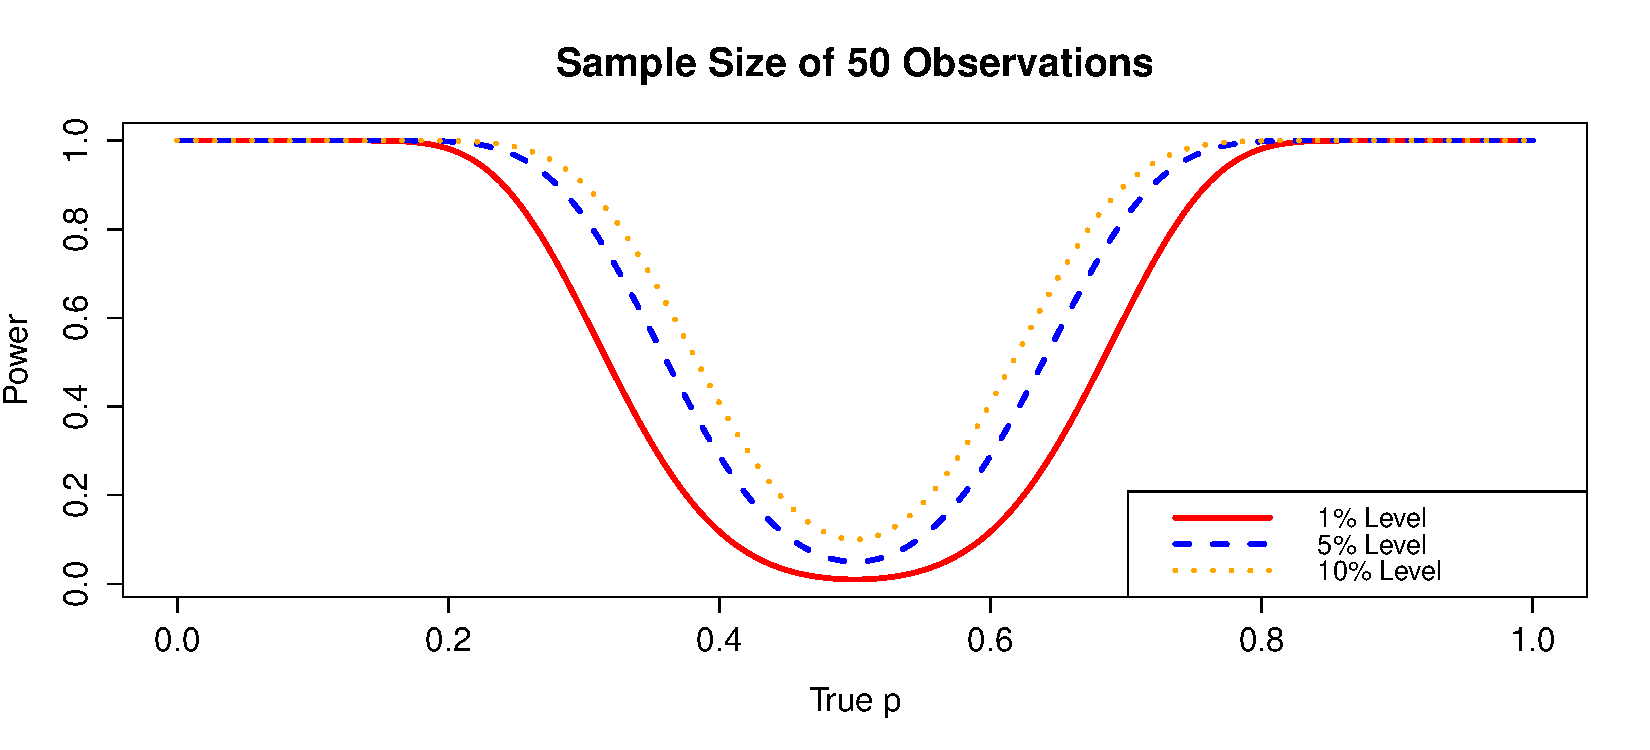
\includegraphics[scale=0.37]{./images/power_change_a}
\end{center}
\end{frame}
%%%%%%%%%%%%%%%%%%%%%%%%%%%%%%%%%%%%%%%%
\begin{frame}
\frametitle{Some Intuition about Power for the Coin Example}
\small
	\begin{itemize}
	\item Equals prob.\ of rejecting false null, i.e.\ convicting a guilty person.
	\item Tells us how large a sample we would need to detect a given discrepancy from ``fairness'' of the coin: $p = 0.5$
		\begin{itemize}
			\item Small deviations from $p=0.5$ unlikely to be detected unless the sample size is large.
			\item Large deviations from $p=0.5$ very likely to be detected even if the sample size is small.
		\end{itemize}
		\item For a \emph{given} degree of ``unfairness'' (deviation from $p = 0.5$)
			\begin{itemize}
				\item Higher significance level ($\alpha$) $\implies$ higher power ($1-\beta$)
				\item Large sample size ($n$) $\implies$ higher power ($1-\beta$)
			\end{itemize}
	\end{itemize}
\end{frame}

%%%%%%%%%%%%%%%%%%%%%%%%%%%%%%%%%%%%%%%%

\begin{frame}
\frametitle{Power More Generally}
	\begin{block}{Power $ = (1 - \beta) = 1 -  P$(Type II Error)}
Chance of detecting an effect given that one exists.
\end{block}
\begin{block}{Power Depends on Four Things}
	\begin{enumerate}
\item Magnitude of Effect: easier to detect large deviations from $H_0$
\item Amount of variability in the population: less variability $\implies$ easier to detect an effect of given size.
\item Sample Size: larger $n \implies$ easier to detect effect of given size
\item Signif.\ Level ($\alpha$): fewer Type I errors $\implies$ more Type II errors
\end{enumerate}
\end{block}
\alert{Go back and compare to factors that affect width of CI...}
\end{frame}
%%%%%%%%%%%%%%%%%%%%%%%%%%%%%%%%%%%%%%%%
% \begin{frame}
% \frametitle{An Important Point}
% For any discrepancy from $p = 0.5$, there is always a sample size large enough to make the power of our test \emph{arbitrarily close to one}. In other words, we can be almost certain to detect an effect, no matter how small, provided that we use a large enough sample. \alert{However, this does not mean that the affect we have found is important}.

% \vspace{2em}
% If it turned out that the true probability of heads was closer to 0.50001 rather than 0.5, should we really care? 
% \end{frame}
% %%%%%%%%%%%%%%%%%%%%%%%%%%%%%%%%%%%%%%%%
\begin{frame}[fragile]
\frametitle{An R Function to Calculate Power For Coin Example}
\footnotesize
	\begin{eqnarray*}
		\mbox{Power}(\alpha, p, n) &=& P\left(Y \leq -c\right) + P\left(Y\geq c\right)\\
			 c &=&\texttt{qnorm}(1 - \alpha/2) \\
			 Y &\sim& N\left(\sqrt{n}(2p-1), 4 p(1-p)  \right)
		 \end{eqnarray*} 

\begin{verbatim}
coin.power <- function(a, p, n){
    c <-  qnorm(1 - a/2)	
    mu <- sqrt(n) * (2 * p - 1) 	
    sigma <- sqrt(4 * p * (1 - p))
    
    less.than <- pnorm(-c, mean = mu, sd = sigma)
    greater.than <- 1 - pnorm(c, mean = mu, sd = sigma)
    power <- less.than + greater.than
    return(power)
}
\end{verbatim}
\end{frame}


%%%%%%%%%%%%%%%%%%%%%%%%%%%%%%%%%%%%%%%%

\begin{frame}[fragile]
\frametitle{Here's Some Code for You to Play Around With}
\footnotesize
You can use the function \texttt{coin.power} to calculate power for specific values of $p, n,$ and $\alpha$
\begin{verbatim}
coin.power(a = 0.05, p = 0.55, n = 100)
coin.power(a = 0.05, p = 0.55, n = 1000)
coin.power(a = 0.1, p = 0.55, n = 100)
coin.power(a = 0.05, p = 0.6, n = 100)
\end{verbatim}
or to make plots similar to those on slide 28
\begin{verbatim}
alternatives <- seq(from = 0, to = 1, by = 0.001)
power <- coin.power(a = 0.05, alternatives, n = 10)
plot(alternatives, power, xlab = `True p', ylab = `Power', type = `l')
\end{verbatim}
Try out different choices for $p,n$ and $\alpha$ and see what you get! I'll post this R code to save typing.

\end{frame}
%%%%%%%%%%%%%%%%%%%%%%%%%%%%%%%%%%%%%%%%

%%%%%%%%%%%%%%%%%%%%%%%%%%%%%%%%%%%%%%%%
% \begin{frame}
% \frametitle{Next Time}
% 	\begin{enumerate}
% 	\item Some final points about Hypothesis testing and CIs
% 	\item Regression Part II
% 	\end{enumerate}
% \end{frame}


\end{document}










































